
\chapter{Results}

\vspace{-1cm}

\section{Key Metric Analysis}

This section presents the results achieved by the navigation system under optimal conditions across various challenging datasets. The analysis focuses on the system's performance in terms of accuracy, efficiency, and generalizability, providing insights into its applicability in real-world UAV navigation scenarios. More information about the testing setup is provided in \ref{chap:Testing}




\subsection{Performance Analysis}

The system's performance across the five diverse datasets—CITY1, CITY2, ROCKY, DESERT, and AMAZON—is evaluated based on Accuracy and Runtime.

\textbf{Accuracy} is assessed in two primary ways:

1. \textit{Absolute Radial Error (RMSE)}: Measured in the estimates radial metres from the ground truth, averaged for the dataset. This metric provides a tangible understanding of the error magnitude and the system's responsiveness to movement size. Additionally, it may be represented per-image, in pixels or in axial components, offering an intuition of error size relative to the fixed resolution of 1920x972 pixels.

2. \textit{Relative Radial Error}: Expressed as the per image Absolute Radial Error as a percentage of the ground truth radial change in distance, averaged for the dataset. The ground truth radial change is the magnitude of the translation vector from the reference image's center to the current image's center, both measured in meters. This normalized metric allows for a clearer understanding of the system's accuracy relative to the movement size. It may also be represented per-image or in axial components.


\textbf{Runtime} is evaluated in three stages:
1. \textit{Mean Add Time (With GNSS)}: The average time required to add one image to the pipeline, including streaming the image and extracting its features. This time determines the system's processing rate while GNSS signals are available after parameter inference has concluded.

2. \textit{Mean Parameter Inference Time (With GNSS)}: The average time needed to infer the pixel-to-meter conversion factor per image. This includes processing the entire pipeline (finding the best match and subsequent transformation estimation) to estimate the UAV's position, and computing linear regression by leveraging the ground truth once at the end of the mode. Adding this to the add time provides the total time to process an image when GNSS is available and parameter inference is active. Inference mode is active for the first five images, since further tests continued to limit the reference image capture rate while producing negligible improvements in accuracy.

3. \textit{Mean Location Inference Time (Without GNSS)}: The average time taken to infer the UAV's location when GNSS signals are lost. Measured per image, this time encompasses processing the entire pipeline to estimate the UAV's position. This metric is critical as it determines how quickly a pilot can correct any path deviations to prevent further drift.
The results demonstrate that the system consistently achieves high accuracy and efficient runtime performance across all datasets. This section provides a detailed analysis of the performance metrics for each dataset, followed by an examination of the sources of error where applicable.

\subsection{Requirements Compliance}

This section provides a concise detailing of the systems ability to meet the outlined requirements, as detailed in \ref{sec:requirements}. Table \ref{tab: Requirements} shows the system's full compliance with the requirements; however, the performance is evaluated in more details in the subsequent sections. 

\begin{table}[H]
    \centering
    \caption{Compliance with Requirements for Radial Error and Processing Time}
    \label{tab: Requirements}
    \begin{tabular}{|c|c|c|c|c|c|}
    \hline
    \textbf{Requirement} & \textbf{CITY1} & \textbf{CITY2} & \textbf{ROCKY} & \textbf{DESERT} & \textbf{AMAZON} \\ \hline
    \makecell{\textbf{Max Radial} \\ \textbf{Error $\leq$ 10\%}} & 0.6356\% & 0.2715\% & 6.2123\% & 0.3516\% & 0.7447\% \\ \hline
    \makecell{\textbf{Max post-GNSS} \\ \textbf{Inference Time $\leq$ 2s}} & 1.3609s & 1.6271s & 1.4374s & 1.8392s & 1.7091s \\ \hline
    \makecell{\textbf{Max with-GNSS} \\ \textbf{Time $\leq$ 5s}} & 2.0377s & 2.1342s & 2.2412s & 2.2418s & 2.3975s \\ \hline
    \end{tabular}
\end{table}
    


\subsection{Results}


This section observes the results, while Section ~\ref{sec:Error Analysis} discusses the sources of error in the system.

In terms of accuracy, as shown in Figures \ref{fig:Accuracy} and \ref{fig:Pixel Accuracy}, all datasets achieved a mean radial error below 2\% of the ground truth distance, a mean pixel error below 1.05 pixels, and a mean meter error below 3.2 meters. Evaluating the percentage error, the datasets' performance, from best to worst, is as follows: CITY2, DESERT, AMAZON, CITY1, and finally, with a significant difference in performance, ROCKY.

Regarding maximum single image errors, the highest error occurred in the ROCKY dataset, with a maximum radial error of 6.21\% of the ground truth distance, corresponding to 27.54 meters or 4.93 pixels.

For runtime performance, as shown in Figure \ref{fig:Runtimeopt}, the mean add (feature extraction) time across datasets was below 0.6 seconds, the mean parameter inference time was below 1.4 seconds, and the mean location inference time was below 1.3 seconds. This indicates that the system maintains real-time performance even while inference mode is on, with the sum of the mean parameter inference and add times being below 2 seconds (with a 5-second requirement), and the location inference time below its requirement of 2 seconds.

Regarding maximum single image runtimes, the system remained under the crucial 2-second threshold following GNSS-signal loss. The system produced runtimes in the with-GNSS phase slightly above 2 seconds while inference mode was active (adding the add time and parameter inference time). When inference mode was off, this runtime stayed below 2s. Over the entire flight, this would be caught up and result in a mean runtime below 2s, well below the 5s requirement. 

\begin{figure}[H]
    \begin{minipage}{0.49\textwidth}
           \centering
        \centering
        \includegraphics[width=\textwidth]{Chapter 5/RESULTPLOTS/newkey/percacc.png}
        \caption{Mean Percentage Error Across Datasets (Movement Size Normalized).}
        \label{fig:Accuracy}
    \end{minipage} \hfill
    \begin{minipage}{0.49\textwidth}
        \centering
        \includegraphics[width=\textwidth]{Chapter 5/RESULTPLOTS/newkey/pixmetacc.png}
        \caption{Mean Pixel and Metre Error Across Datasets.}
        \label{fig:Pixel Accuracy}
    \end{minipage}
\end{figure}


\begin{figure}[H]
    \centering
    \includegraphics[width=0.6\textwidth]{Chapter 5/RESULTPLOTS/newkey/pixmetacc.png}
    \caption{Mean and Max Runtime Performance Across Datasets.}
    \label{fig:Runtimeopt}
\end{figure}



\subsection{Visual Analysis}

Figures \ref{fig:Flight Path ROCKY} and \ref{fig:Flight Path DESERT} illustrate the actual versus estimated flight paths of the UAV in the ROCKY and DESERT datasets, respectively. Despite the ROCKY dataset being the worst performer, the system maintains a highly accurate flight path when looking on a broader scale, demonstrating that the error is negligible on a global scale. In reality, this error is sufficiently low that the pilot can control the UAV and prevent further drift on a variety of terrains.

\begin{figure}[H]
    \centering
    \begin{minipage}{0.45\textwidth}
        \centering
        \includegraphics[width=0.9\textwidth]{./Chapter 5/GPSpaths/PathCity1.png}
        \caption{Flight Path of UAV in Rocky Dataset (Worst)}
        \label{fig:Flight Path ROCKY}
    \end{minipage}\hfill
    \begin{minipage}{0.45\textwidth}
        \centering
        \includegraphics[width=0.9\textwidth]{./Chapter 5/GPSpaths/PathCity2.png}
        \caption{Flight Path of UAV in Desert Dataset (Best).}
        \label{fig:Flight Path DESERT}
    \end{minipage}
\end{figure}


Figure \ref{fig:Matches_CITY2} presents examples of the top 50 worst matches, post-filtering, in the CITY2 dataset. This clearly indicates the reliability of matches on a broader scale.

\begin{figure}[H]
    \centering
    \includegraphics[width=0.8\textwidth]{Chapter 5/RESULTPLOTS/appfigs/matches.png}
    \caption{Matches Between Two Images in CITY2 Dataset.}
    \label{fig:Matches_CITY2}
\end{figure}



Figure \ref{fig:Overlay_CITY2} shows the overlay of two images in the CITY2 dataset after rotation and translation. This visual representation demonstrates the system's ability to find the correct transformation between images. The borders are due to rotating off-canvas and canvas borders. As visible, the system aligns the two images almost perfectly. Notably, near the outer edges of the overlaid section, there are areas of slight blur, indicating the effect of relative velocity differences between pixels in the center and edges of the image due to the angle at which the light sources at the edge of the field of view are incident on the camera. Although a minor source of error in this study, cameras with larger degrees of fisheye distortion may experience more significant errors in these areas.



\begin{figure}[H]
    \centering
    \includegraphics[width=0.4\textwidth]{Chapter 5/RESULTPLOTS/appfigs/OVERLAY.png}
    \caption{Overlay of Two Images in CITY2 Dataset.}
    \label{fig:Overlay_CITY2}
\end{figure}



The heatmap in Figure \ref{fig:Heatmap_XY_Dev} illustrates the distribution of pixel deviations in the X and Y directions across the datasets. For spatial conciseness, some axial values are omitted, and the values are quantized into bins, meaning they are not exactly off by the pixel bin they are in. This visualization provides an intuitive understanding of the pixel error distribution and any potential axial bias. As shown, the errors are distributed relatively evenly across both axes, indicating no significant axial bias in the system. Moreover, the majority of errors are below 2 pixels, demonstrating the system's robustness and accuracy in localization estimates. The largest radial error, as noted in Table \ref{fig:Heatmap_XY_Dev}, is 4.9199 pixels. While this error is relatively small, the sources of these errors are discussed in the following section.




\begin{figure}[H]
    \centering
    \includegraphics[width=0.4\textwidth]{Chapter 5/RESULTPLOTS/XYHEAT.png}
    \caption{Heatmap of Pixel Deviations in X and Y Directions}
    \label{fig:Heatmap_XY_Dev}
\end{figure}



\subsubsection{Analysis of Identified Sources of Error}
\label{sec:Error Analysis}

The system’s maximum error was observed to be 6.2\% of the UAV displacement on the ROCKY dataset. Additionally, notable outliers were detected in the CITY1 and AMAZON datasets, with maximum errors of 0.64\% and 0.74\%, respectively. Below, the sources of these errors are analyzed, highlighting their prevalence across all datasets and their amplified effects in specific cases.

\textbf{Differences in Step Size:}
Although the mean performance across all datasets is relatively low, a significant outlier was observed in one image in the ROCKY dataset. This is attributed to the step, or displacement, size of that image relative to its best reference match. The radial translation between these images is around 873 pixels—the largest step size by a considerable margin in all datasets. This step decreased the mutual information overlap to 59.4\%, the lowest among all datasets, leading to a higher error of 6.2\% of the UAV displacement. It is thereby crucial to maximize the path overlap to maintain a high level of accuracy, as it forms the primary reason for poor performance in the ROCKY dataset.


\textbf{Quantization Effects:}  
When images are captured from slightly different positions, sub-pixel shifts cause feature edges to distort. At a fixed resolution, any information smaller than a pixel is averaged, leading to potential inaccuracies. For large features, the impact of this distortion is minimal relative to the feature size. However, smaller features experience significant boundary distortions, causing high levels of descriptor and keypoint inaccuracies. This effect is exacerbated at higher altitudes where features are predominantly small, impacting descriptor fidelity and keypoint precision. The CITY datasets, with their dense, small-scale features, are especially affected, causing increased sub-pixel errors. While CITY2 experiences sub-pixel shifts as well, its simpler frame-to-frame translations (without significant rotation) help reduce overall error, making the effect less pronounced.

\textbf{Depth and Perspective Variations:}  
Google Earth’s 3D terrain model introduces changes in perspective and ground height as images are captured from various positions. These variations are intensified by significant altitude changes in the landscape. The ROCKY dataset, characterized by pronounced height differences in mountainous areas, demonstrates the effects of these perspective distortions and scale discrepancies.

\textbf{Homogeneous and Repetitive Terrain:}  
The effectiveness of keypoint detection relies on the presence of unique, high-contrast features. Similarly, the accuracy of matching depends on whether the local environment surrounding a feature is sufficiently distinct. In homogeneous and repetitive environments, such as the AMAZON dataset, feature detectors struggle to identify a diverse set of keypoints, and matchers face challenges in selecting correct correspondences. Modern computer vision techniques mitigate this issue to a large extent, but in highly repetitive terrains, even these advanced methods encounter marginal difficulties.

\textbf{Variability in Terrain and Environmental Conditions:}  
Each dataset’s terrain has unique attributes, such as the density of good features and the uniqueness of keypoints. Optimal feature counts vary with terrain type; however, this study applied a uniform target number of keypoints and matches across all datasets. This static approach does not fully account for the variability in feature distribution and environmental conditions, leading to generalized performance rather than terrain-specific optimization.

\textbf{Optical Distortion Effects:}  
Camera lenses cause distortion, particularly at the edges of the frame. This occurs because light from the edges enters the lens at steeper angles compared to the center, resulting in different perceived motion. This change in angle affects how features move across frames, making the outer pixels appear to move slower than those at the center. This non-uniform movement can lead to discrepancies in pixel displacement, impacting keypoint detection and matching accuracy. 

\textbf{Algorithmic Limitations:}  
The image processing and matching algorithms employed have intrinsic constraints, particularly under challenging conditions or when handling repetitive features. Optimized for computational efficiency, these algorithms may not capture every image feature perfectly, contributing to potential errors in feature detection and matching.


\section{Adverse Conditions Evaluation}

To ensure the system's robustness and practical viability, it is essential to evaluate its performance under various challenging conditions. This section presents tests conducted under dynamically varying lighting conditions, reduced resolution, and low reference image overlap (mutual pixels). These tests were selected for their practical relevance and current applicability. The results provide insights into the system's performance under adverse conditions and highlight potential areas for improvement.

\subsection{Low Resolution Testing}

This section evaluates the system's performance under varying resolution factors, relative to the original 1920x972 resolution. The analysis focuses on the trade-off between navigational accuracy and computational efficiency as the resolution decreases. The goal is to identify whether the system can maintain performance in scenarios where the UAV has limited power and computational resources available and can only operate at lower resolutions.

\subsubsection{Results}

The results, as shown in Figures \ref{fig:Resolution_ACC} and \ref{fig:Resolution_Time} indicate that the system maintains a stable performance with minimal changes in accuracy until the resolution is reduced to an absolute resolution of 336x221. At this point, there is a sharp increase in error in the AMAZON dataset, indicating that the system's accuracy becomes significantly compromised. Interestingly, the accuracy remains relatively constant down until a certain resolution, suggesting algorithmic robustness to lower levels of detail. 

In terms of runtime, the location inference time decreases as the resolution decreases. A reduction of resolution by half, to 960x486, results in slightly less than a 50\% decrease in runtime. This decrease is due to the reduced number of features and matches possible, leading to a lower computational load. The systems accuracy is not compromised at this resolution. 

\begin{figure}[H]
    \centering
    \begin{minipage}{0.48\textwidth}
        \centering
        \includegraphics[width=0.9\textwidth]{Chapter 5/RESULTPLOTS/lowres/lowresacc.png}
        \caption{Radial (\%) Error vs Resolution Factor}
        \label{fig:Resolution_ACC}
    \end{minipage}\hfill
    \begin{minipage}{0.48\textwidth}
        \centering
        \includegraphics[width=0.9\textwidth]{Chapter 5/RESULTPLOTS/lowres/lowrestime.png}
        \caption{Location Inference Time (s) vs Resolution Factor}
        \label{fig:Resolution_Time}
    \end{minipage}
\end{figure}


\subsubsection{Conclusion}

As evaluated, the system can maintain stable performance at resolutions a slight offset above 336x221, with minimal changes in accuracy. However, below this resolution, the system's accuracy becomes significantly compromised, leading to a sharp increase in error. The system's runtime also decreases linearly as the resolution decreases, with an almost 50\% reduction in runtime observed at a resolution of 960x486 while maintaining performance. This indicates that the system can operate effectively at lower resolutions, providing a viable solution for UAVs with limited computational resources.


\subsection{Mutual Information Testing}

This section evaluates the system's performance under reduced mutual information, which is the number of pixels shared between images, as a percentage of the image size. The system's accuracy and runtime are analyzed as the mutual information decreases, providing insights into the trade-off between navigational accuracy and computational efficiency. The results aim to identify the minimum mutual information required for reliable navigation and real-time performance.

\subsubsection{Methodology}

To emulate a decrease in mutual information, images are progressively cropped and the mutual information is calculated for each instance. The CITY2 dataset is utilized, focusing exclusively on translational changes which simplifies the mutual pixel calculation to the difference between the image size and translation vector. Cropping is performed at a rate of 50 pixels per iteration, scaled up in the x direction by the aspect ratio, alternating between x and y crops. Since translation vectors vary between images, only the mutual information of the bottleneck image (the one with the lowest mutual information) is shown for each iteration to maintain visual brevity.

\subsubsection{Results}

The accuracy plot in Figure \ref{fig:Mutual_Information_ACC} indicates that the error remains almost constant until the overlap drops below approximately 30\%, at which point the error starts to increase. It is important to note that below the lowest tested value, the mutual information of the bottleneck image was below 0, hence the error from thereon is not shown. Interestingly, the error decreases again after a significant increase at an even lower overlap. However, this reduction is unreliable and results from reductions in non-mutual information causing a coincidental high density of good matches, despite the low number of mutual pixels. Therefore, extremely low levels of mutual information cannot be relied upon for consistent accuracy. Maintaining an overlap above 30\% ensures stable and accurate navigation. 

The runtime plot in Figure \ref{fig:Mutual_Information_Time} shows an underlying linear trend in runtime and mutual information. As expected, the runtime decreases with a decrease in mutual information, as the number of features and matches decreases with the image size, reducing the computational load. This rate is slightly above 0.1 s per 10\% reduction in mutual information. This decrease is moderate and measures may be taken to decrease the field of view of the camera when the UAV is close to the path, to reduce the computational load, but this will not result in a large runtime boost.

\begin{figure}[H]
    \centering
    \begin{minipage}{0.48\textwidth}
        \centering
        \includegraphics[width=\textwidth]{Chapter 5/RESULTPLOTS/MUTUAL_ACC.png}
        \caption{Mutual Information vs Mean Error Percentage.}
        \label{fig:Mutual_Information_ACC}
    \end{minipage} \hfill
    \begin{minipage}{0.48\textwidth}
        \centering
        \includegraphics[width=\textwidth]{Chapter 5/RESULTPLOTS/MUTUAL_TIME.png}
        \caption{Mutual Information vs Mean Localization Time.}
        \label{fig:Mutual_Information_Time}
    \end{minipage}
\end{figure}

\subsubsection{Conclusion}
The results show the UAV was able to maintain accuracy until the mutual information dropped below 30\%. The runtime decreased with a decrease in mutual information, as expected; however, this runtime is not necessarily worth the potential for instability. Minor crops can be used once the path is found, but the occasional cross-referencing with the full image would be essential to be sure of the UAV's position. 

\subsection{Low-Light Testing}

In the context of UAV navigation, long missions may require the UAV to return along the outbound path at a significantly different time to the outbound journey. In this test, the reference image lighting conditions are altered relative to that of the current image. This adds an extra layer of difficulty to the task above simply changing all of the images to low-light would not fully capture; however, the ability to operate under low-light conditions is implicitly tested here too. 

Since darker images have less uniqueness and contrast, the number of features found will become too low if the dynamic detector threshold is adjusted to target a specific number of keypoints for day time conditions. Therefore, it is adjusted for the simulated night-time conditions, acknowledging this more lenient threshold leads to more keypoints and subsequently higher runtime. In practice, the detector threshold should be recalculated from time to time to ensure a consistent number of keypoints are found across all images at different times. 


\subsubsection{Methodology}

This section evaluates the robustness of the navigation method under simulated evening and nighttime conditions across five datasets: CITY1, CITY2, ROCKY, DESERT, and AMAZON. The following parameters visible in table \ref{tab:lighting_params} are used to simulate the lighting effects for the different conditions, with day applying no effects. It is noted that night-time conditions are simulated through darkening and adding noise, rather than actual night-time conditions which include dynamic changes in lighting. The alpha parameter controls contrast while Beta reduces the brightness of the image. Noise sigma, or standard deviation, adds Gaussian noise to mimic low-light imperfections. Weight balances the processed image and Gaussian noise effect for realism in night simulations, with higher values implying most of the image remains the same. To ensure that all values are visible on the plot, percentage increase from daytime error is used alongside a logarithmic scale on the y-axis. 

    \begin{table}[H]
        \centering
        \begin{tabular}{|c|c|c|c|c|}
        \hline
        \textbf{Effect} & \makecell{\textbf{Alpha} \\ \textbf{(Contrast)}} & \makecell{\textbf{Beta} \\ \textbf{(Brightness)}} & \textbf{Noise Sigma} & \textbf{Weight (main)} \\
        \hline
        Early Evening & 0.7 & -15 & 10 & {0.97} \\
        Late Evening & 0.6 & -30 & 15 & {0.95} \\
        Late Night & 0.5 & -50 & 20 & {0.92} \\
        \hline
        \end{tabular}
        \caption{Parameter Settings for Different Lighting Effects reproduced from \cite{GoogleEarth}.}
        \label{tab:lighting_params}
    \end{table}
    
        
Representative examples from the CITY1 dataset illustrate these conditions:
\begin{figure}[H]
    \centering
    \begin{minipage}{0.24\textwidth} % Adjust width as necessary
        \centering
        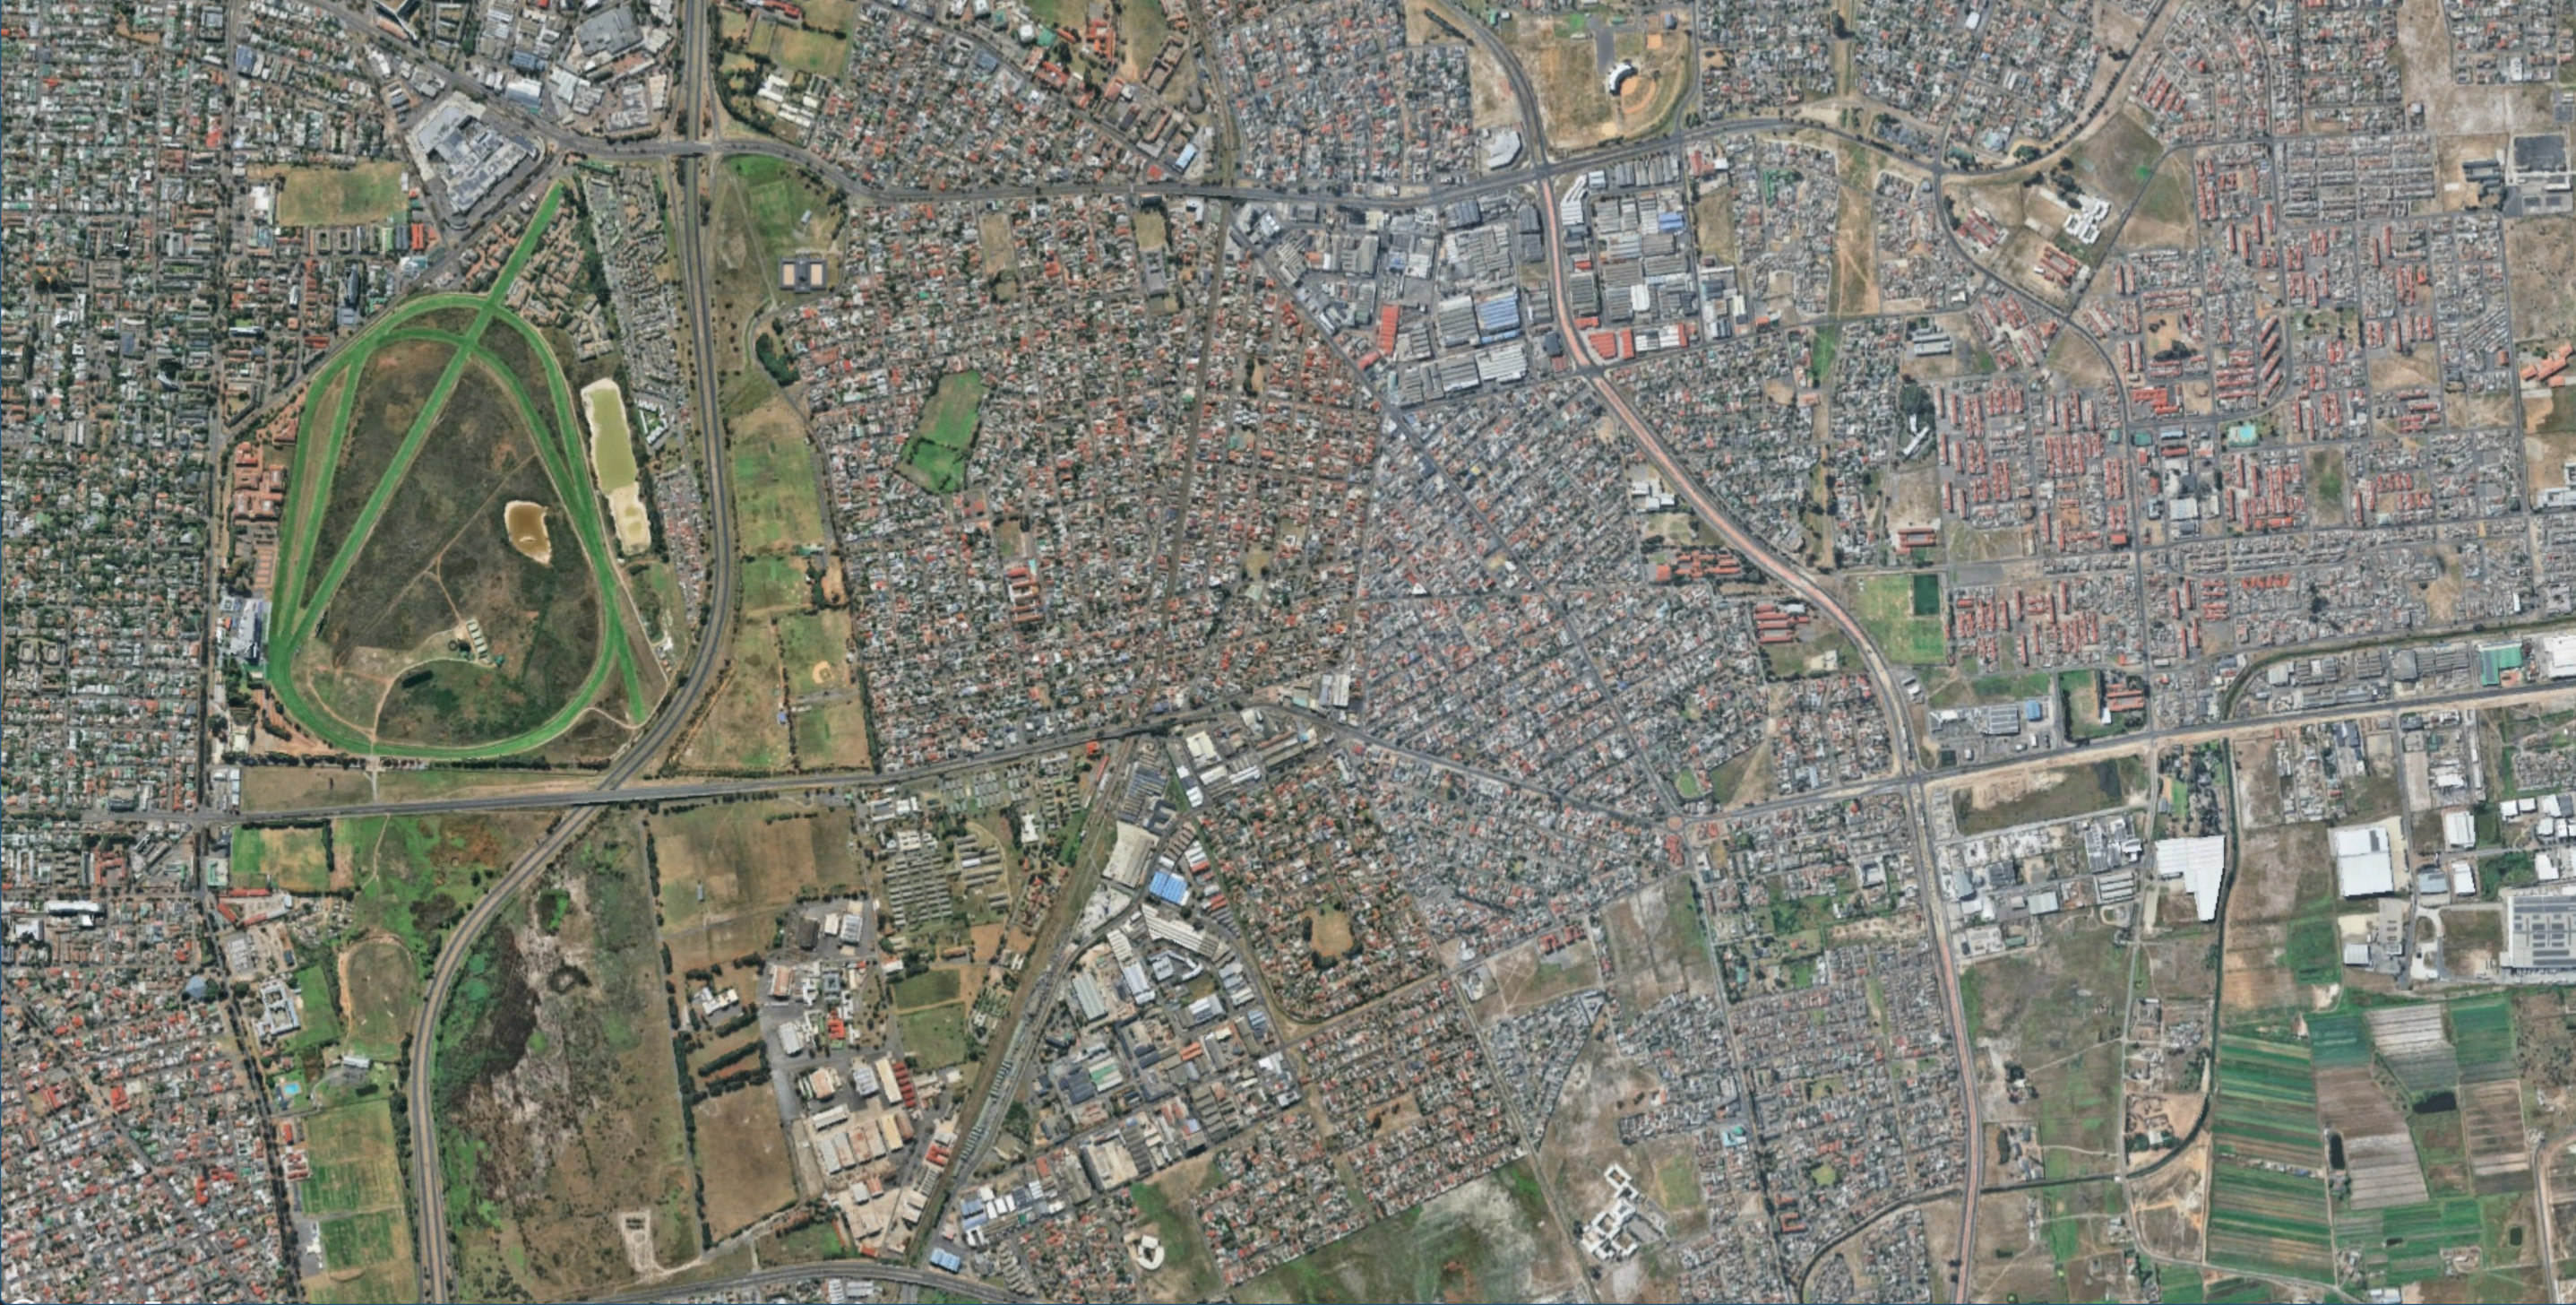
\includegraphics[width=\textwidth]{Chapter 5/RESULTPLOTS/lighting/CPTdayeg.png}
        \caption{Daytime.}
        \label{fig:Day_CPT}
    \end{minipage}\hfill
    \begin{minipage}{0.24\textwidth} % Adjust width as necessary
        \centering
        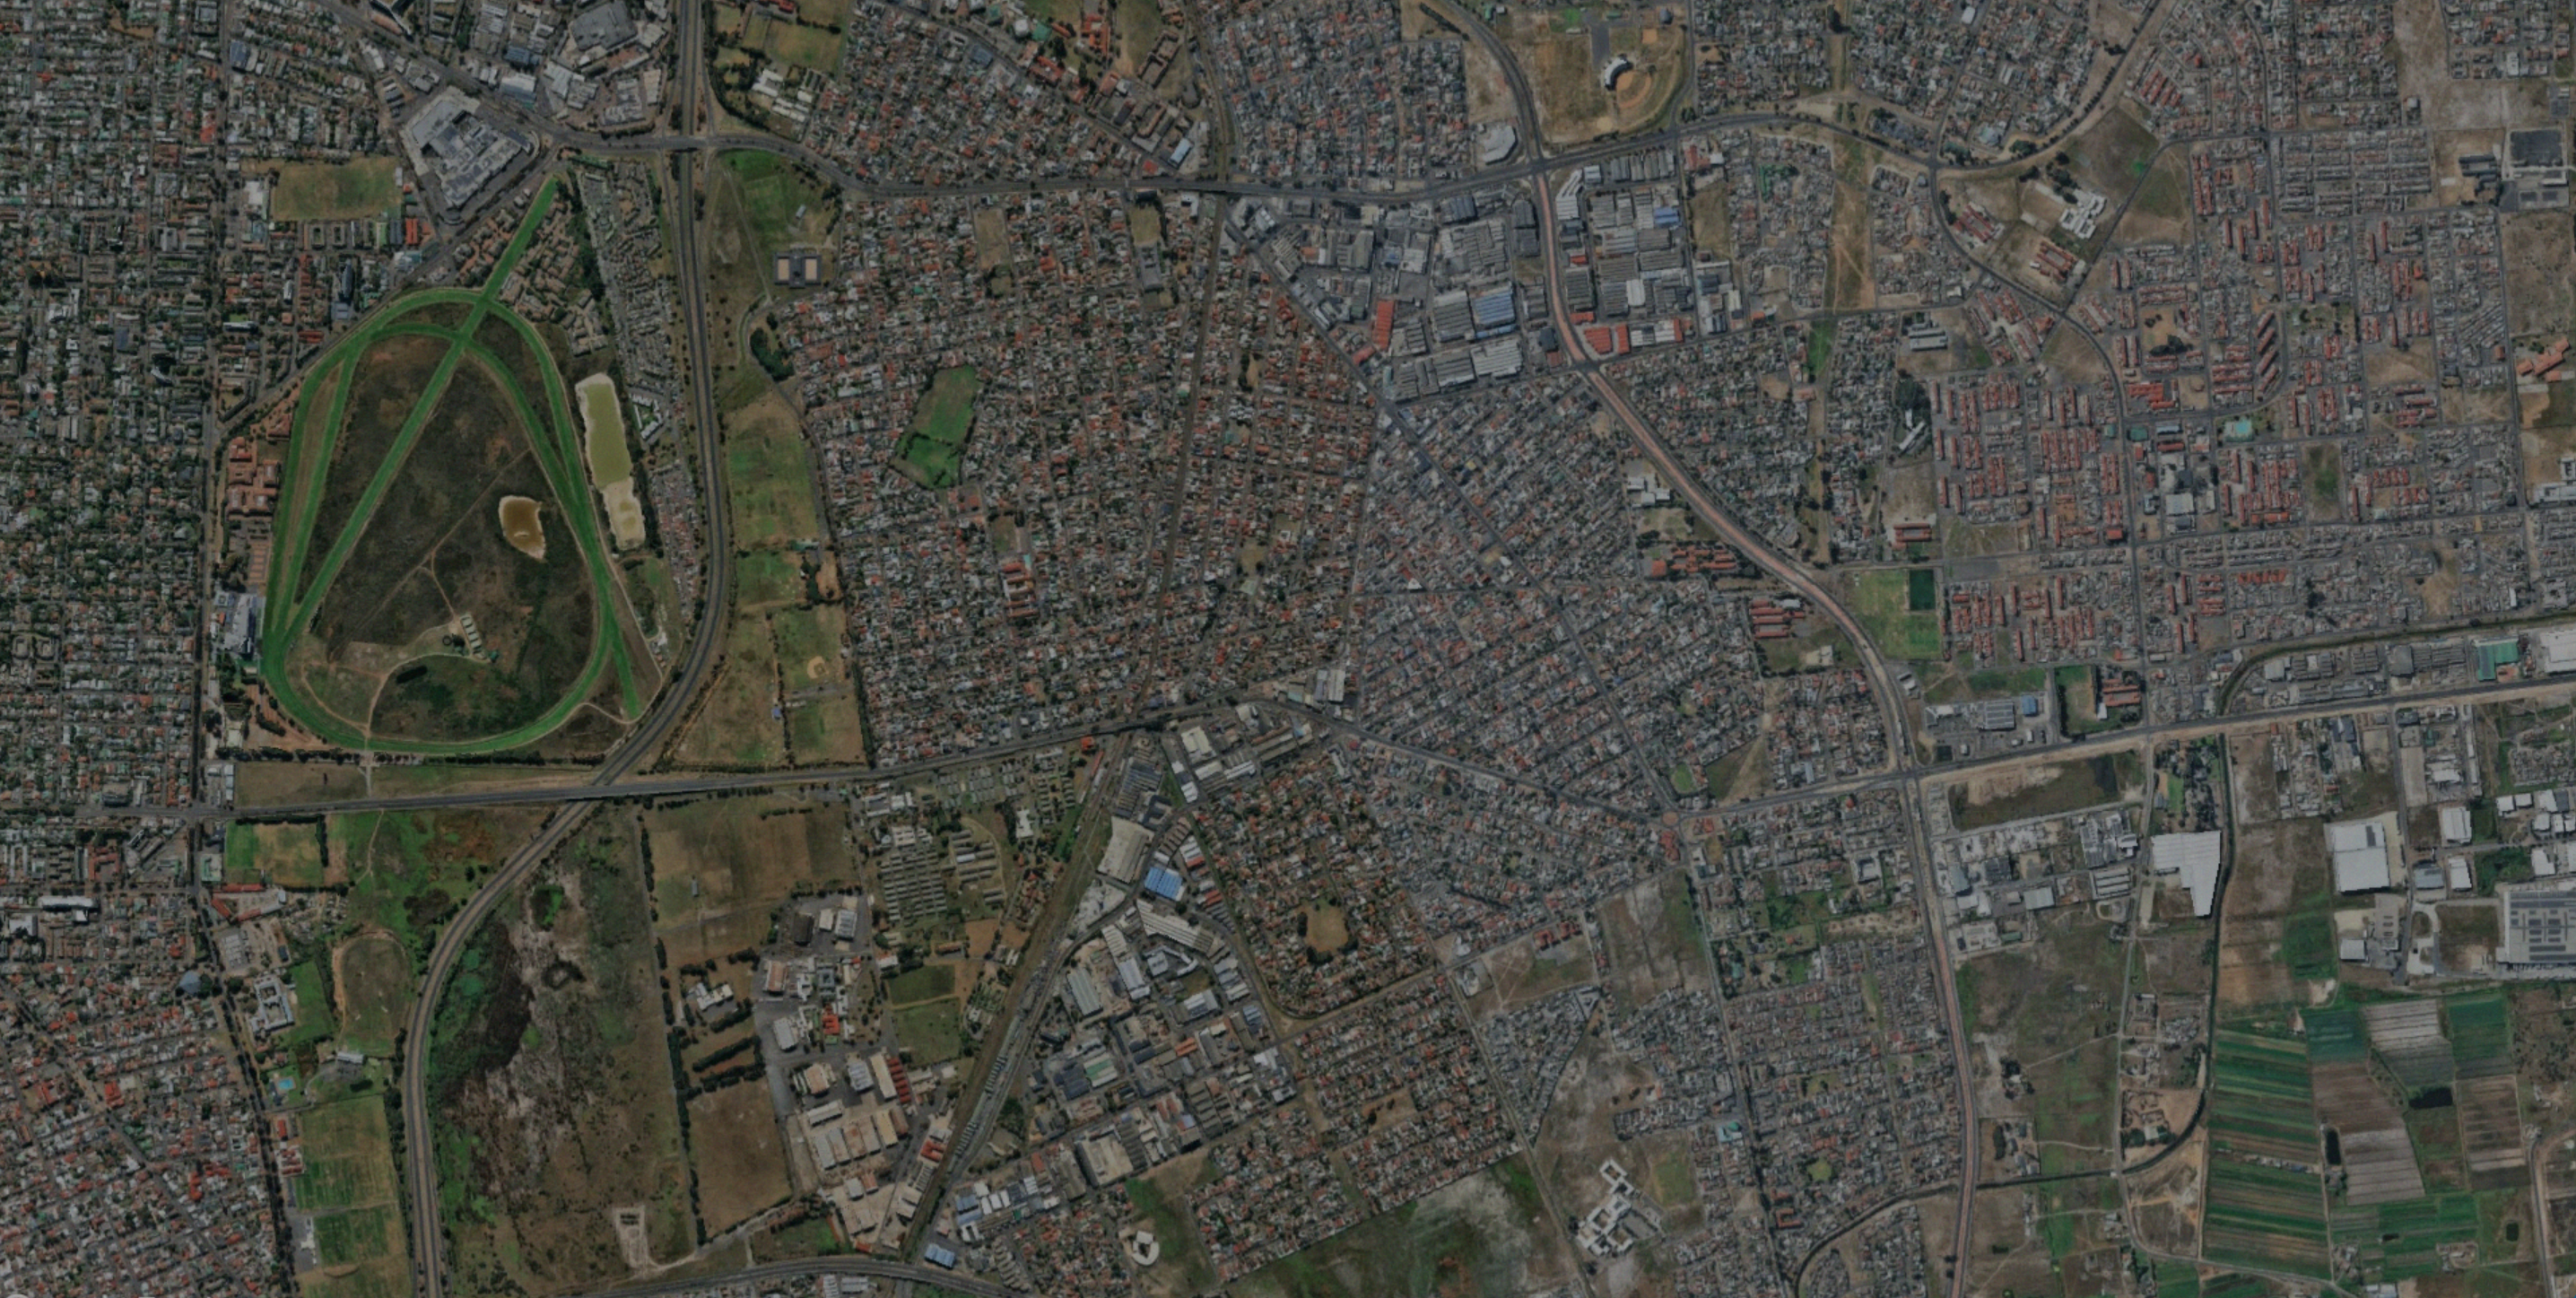
\includegraphics[width=\textwidth]{Chapter 5/RESULTPLOTS/lighting/CPTearlyeveningeg.png}
        \caption{Early Evening.}
        \label{fig:Early_Evening_CPT}
    \end{minipage}\hfill
    \begin{minipage}{0.24\textwidth} % Adjust width as necessary
        \centering
        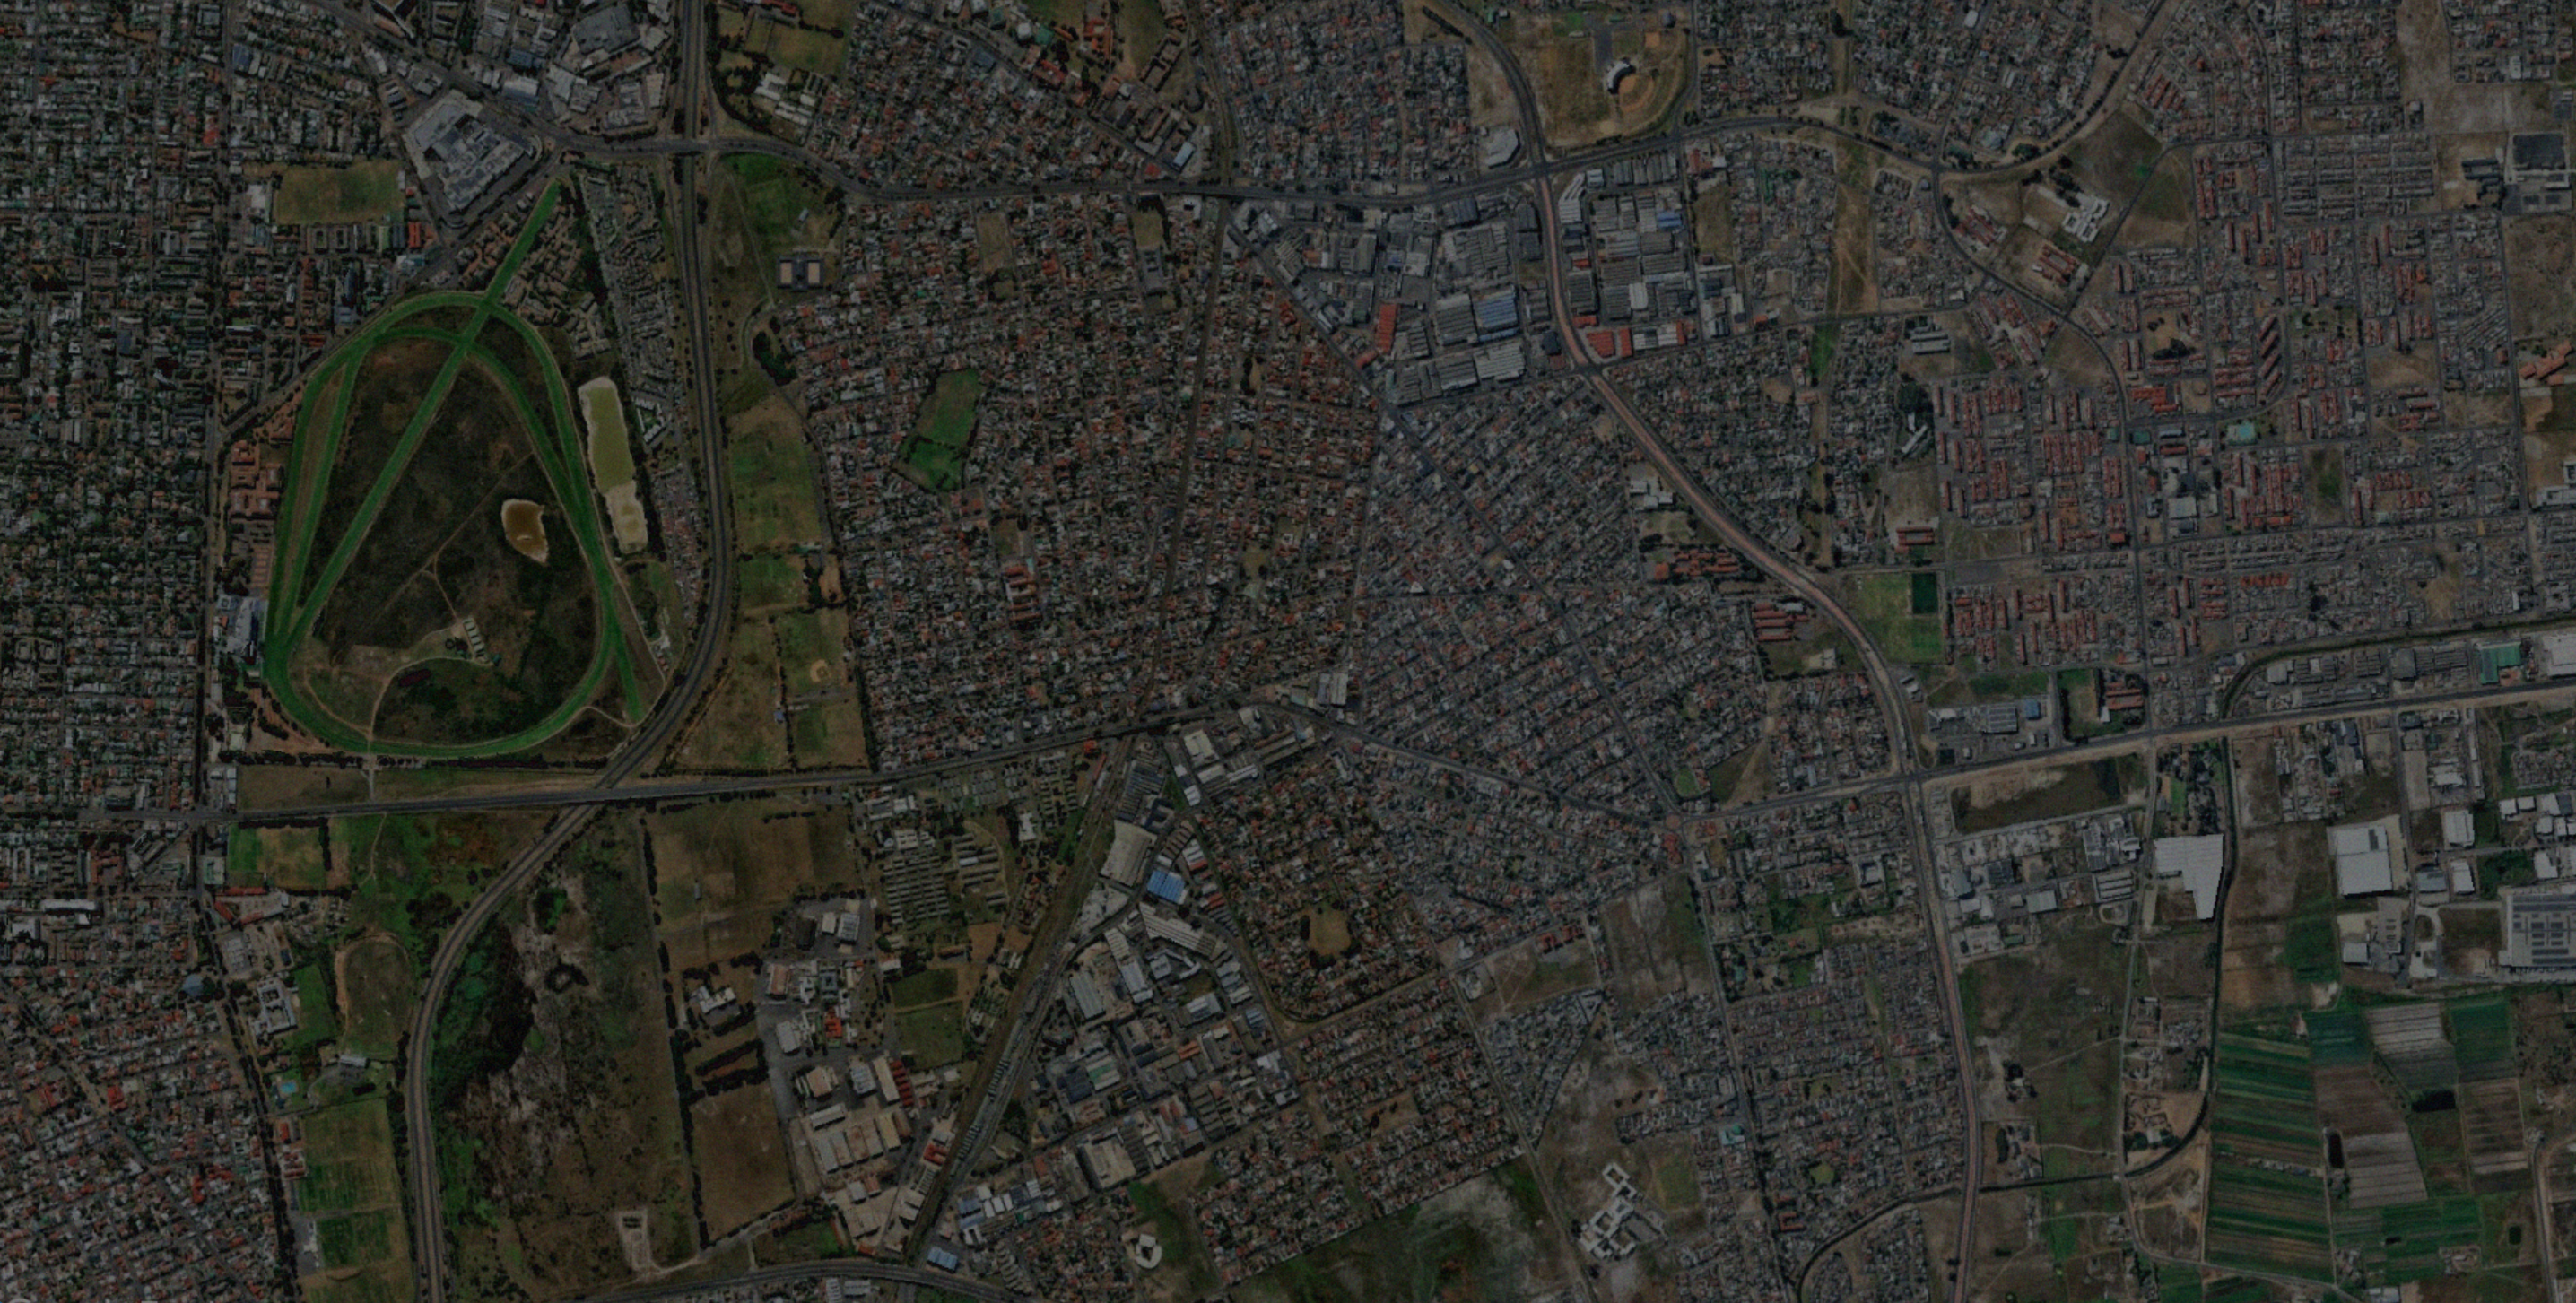
\includegraphics[width=\textwidth]{Chapter 5/RESULTPLOTS/lighting/CPTlateeveningeg.png}
        \caption{Late Evening.}
        \label{fig:Late_Evening_CPT}
    \end{minipage}\hfill
    \begin{minipage}{0.24\textwidth} % Adjust width as necessary
        \centering
        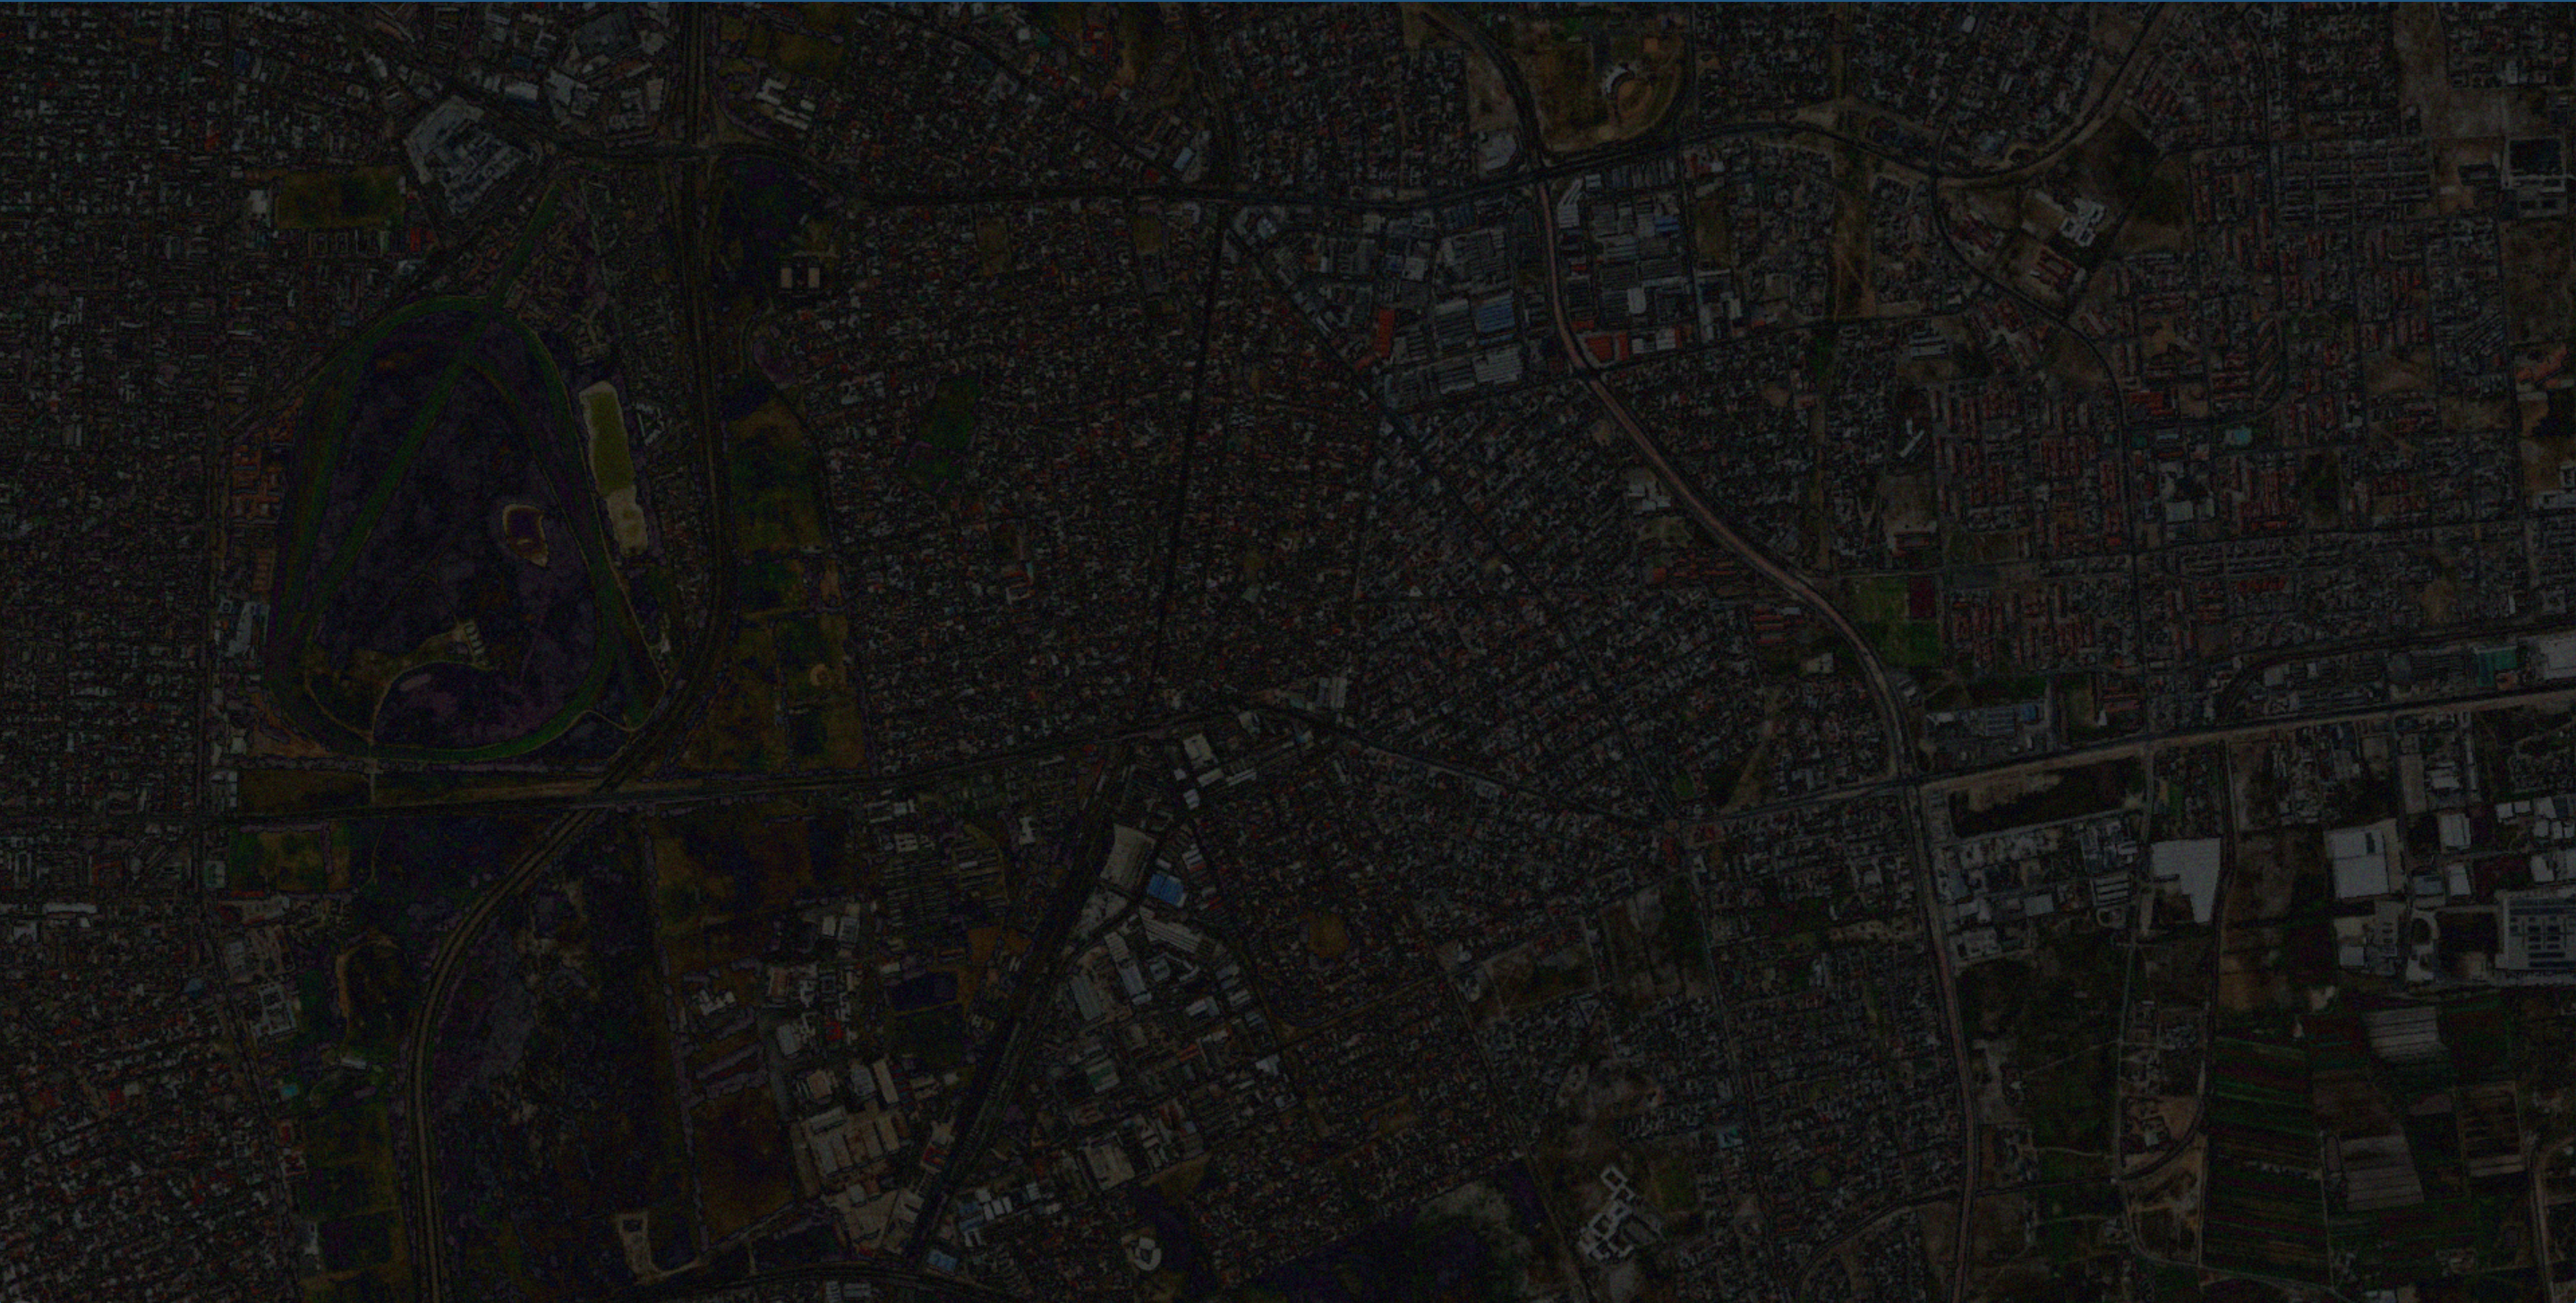
\includegraphics[width=\textwidth]{Chapter 5/RESULTPLOTS/lighting/CPTnighteg.png}
        \caption{Night-Time.}
        \label{fig:Night_CPT}
    \end{minipage}
    
    \caption*{{Simulated Low-Light Conditions in Cape Town reproduced from \cite{GoogleEarth}.}}
    \label{fig:Lighting_CPT}
\end{figure}


\subsubsection{Results}


Figure \ref{fig:night_evening_rmse} illustrates the increase in percentage error following each time change across datasets, relative to the daytime performance. 

The CITY1 dataset shows the smallest increase in error across all conditions, maintaining an error increase under 10\%. CITY2 follows with slightly higher increases in error as lighting conditions become more challenging. This could be attributed to the dataset's minimal rotations, which do not implicitly remove non-mutual information and thereby reduce false positives under difficult conditions, as is the case with the CITY1 dataset. The strong performance of the CITY datasets can be attributed to their dense feature environments with numerous high-contrast elements. However, in real-world scenarios, city lights—unaccounted for due to dataset limitations—could introduce dynamic changes impacting accuracy, especially if they occupy a significant portion of the view.

The ROCKY dataset ranks third in performance, with the DESERT and AMAZON datasets experiencing the largest increases in error. The substantial error rise in these datasets is due to their already sparse environments becoming even more feature-poor under low-light conditions, significantly increasing navigation error. The midnight and late evening settings are particularly challenging, with errors exceeding 100 times the baseline daytime error in these sparse environments.


\begin{figure}[H]
    \centering
    \includegraphics[width=0.55\textwidth]{Chapter 5/RESULTPLOTS/lighting/lightresults.png}
    \caption{Mean percentage increase in error under nighttime and evening conditions.}
    \label{fig:night_evening_rmse}    
\end{figure}

\subsubsection{Conclusion}

Despite the high relative error percentages, the actual error is only realizable when relative to the ground truth distances, not the baseline percentage error. In all datasets, this error is below 5\% of the mean ground truth distance between compared images in the dataset. In denser environments like the CITY datasets, errors remain under 2\% across all lighting conditions. For sparser environments, it is important to mitigate illumination changes during image capture, although the pipeline demonstrates robustness to moderate changes in illumination.


\subsection{Static Tilt}
In practice, the camera may not be facing perfectly downwards. This test evaluates the system's performance under a static forward tilt, in this case pitch, of 7 degrees, exceeding the typical offset a camera may experience due to improper mounting. Radial Error is used in metres for a physical understanding of the system performance with and without the tilt.

As visible in table \ref{tab:tilted_camera}, the system maintains a mean error below 26 meters across all datasets during tilt, with the effect varying depending on the mean ground distance - and thereby the perspective change. The system's robustness to camera tilts is evident, with the error comparable to that without the tilt. This indicates that the system can effectively handle static tilts.

\begin{table}
    \centering
    \caption{Accuracy Results of Tilted Camera Test}
    \label{tab:tilted_camera}
    \begin{tabular}{|c|c|c|c|c|c|}
    \hline
    \textbf{Metric} & \textbf{CITY1} & \textbf{CITY2} & \textbf{ROCKY} & \textbf{DESERT} & \textbf{AMAZON} \\ \hline
    \makecell{\textbf{With Tilt} \\ \textbf{Error (m)}} & 11.13 & 12.04 & 17.20 & 25.11 & 14.53 \\ \hline
    \makecell{\textbf{No Tilt} \\ \textbf{Error (m)}} & 4.80 & 2.76 & 5.88 & 2.36 & 2.53 \\ \hline
    \makecell{\textbf{Ground} \\ \textbf{Height (km)}} & 6.78 & 5.21 & 5.14 & 5.00 & 5.70 \\ \hline
    \end{tabular}

\end{table}



\section{Results Conclusion}

The results presented in this chapter confirm that the system meets the accuracy and time requirements established in the objectives. The system demonstrated consistent and strong accuracy and runtime performance across various datasets, including sparse-feature environments, showcasing its ability to generalize effectively. Additionally, in reality, once the path is found, there will be significantly less translation between the current and reference images, leading to a lower error ceteris 
paribus.

Further, the applied stress tests showed the pipelines invariance to low resolution, low mutual information, static camera tilts, and low-light conditions, with the system maintaining stable performance under these adverse conditions. These results underscore the system's versatility and effectiveness in real-world UAV navigation scenarios, providing a reliable and efficient solution for autonomous navigation.

However, it is noted that sparse datasets do not perform optimally under large variations in lighting, and that a path overlap above 60\% is critical to maintain errors under 5\% of the UAV displacement. 

Overall, the system has proven to be a versatile and effective solution for UAV navigation, showing remarkable potential to sustain operation under a wide range of operational challenges and environmental conditions.

